\documentclass[10pt]{article}
% Packages
\usepackage[utf8]{inputenc}
\usepackage{amsmath}
\usepackage{amssymb}
\usepackage{multicol}
\usepackage[landscape, total={10.8in,8in}]{geometry}
\usepackage{blindtext}
\usepackage{graphicx}
\usepackage{tikz}
\usepackage{enumitem}
\usepackage{array}
\graphicspath{ {./images/} }
% Page formatting
\pagenumbering{gobble}
\parindent=0pt
% Symbols
\newcommand{\C}{{\mathbb C}}
\newcommand{\N}{{\mathbb N}}
\newcommand{\R}{{\mathbb R}}
\newcommand{\Z}{{\mathbb Z}}
\newcommand{\ep}{\varepsilon}
\newcommand{\EP}{\mathcal{E}}
\newcommand{\ihat}{\hat{i}}
\newcommand{\jhat}{\hat{j}}
\newcommand{\khat}{\hat{k}}
% Heading
\newcommand\sectionheading[1]{\begin{center}\large{\textbf{#1}}\end{center}\normalsize}
\newcommand\heading[1]{\medskip\textbf{#1}\medskip}
% \newcommand\heading[1]{\textbf{#1}}

\begin{document}

\begin{center}
    \huge{\textbf{PHYS 158 Formula Sheet}}
\end{center}

\begin{multicols*}{3}

\sectionheading{Mechanical Waves}

\heading{Periodic Waves}

\[T=\frac1f \qquad \omega = 2\pi f \qquad \omega = \frac{2\pi}{T}\]

\[v=\lambda f\]

\heading{Sinusoidal Wave}

Motion in $+x$:

\[y(x,t)=A\cos(kx-\omega t) \qquad k=\frac{2\pi}{\lambda} \qquad \omega=2\pi f\]

\heading{Speed of Wave on String}

\[v=\sqrt{\frac{F}{\mu}} \qquad \mu=\frac{m}{L}\]

\heading{Standing Wave on String}

\[\lambda_n=\frac{2L}{n} \qquad f_n=\frac{nv}{2L}=nf_1 \qquad (n=1,2,3,\ldots)\]

\sectionheading{Sound Waves}

\heading{Pipes}

Open end: pressure node, displacement antinode

Closed end: pressure antinode, displacement node

Open Pipe
\[f_1=\frac{v}{2L} \qquad f_n=\frac{nv}{2L}=nf_1 \qquad (n=1,2,3,\ldots)\]

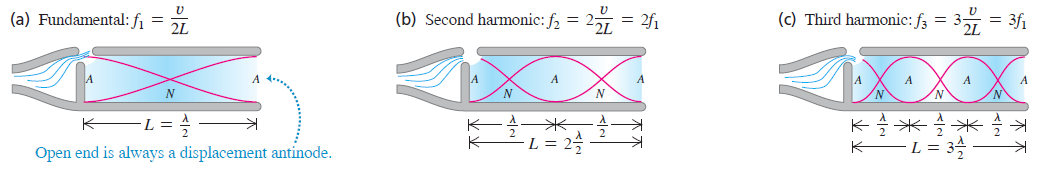
\includegraphics[scale=0.3]{images/fs_open_pipe.png}

Closed Pipe 
\[f_1=\frac{v}{4L} \qquad f_n=\frac{nv}{4L}=nf_1 \qquad (n=1,3,5,\ldots)\]

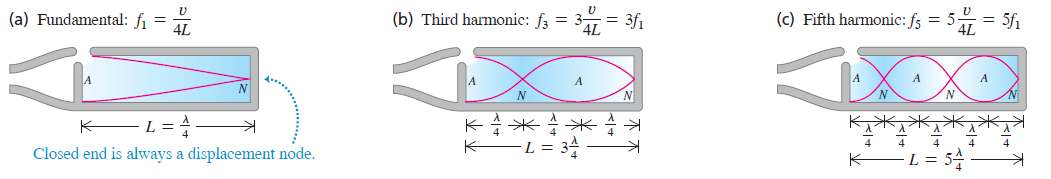
\includegraphics[scale=0.3]{images/fs_closed_pipe.png}

\heading{Beats}

\[f_{\text{beat}}=f_a-f_b\]

\sectionheading{Interference}

Coherent: same $f$ and constant $\phi$ relationship

\heading{Sources in Phase}

Constructive interference:

\[r_2-r_1=m\lambda \qquad (m=0,\pm 1, \pm2, \ldots)\]

Destructive interference:

\[r_2-r_1=(m+\tfrac12)\lambda \qquad (m=0,\pm 1, \pm 2, \ldots)\]

\heading{Two Source Interference}

Bright regions (constructive):

\[d\sin\theta=m\lambda \qquad (m=0,\pm 1,\pm 2,\ldots)\]

Dark regions (destructive):

\[d\sin\theta=(m+\tfrac12)\lambda \qquad (m=0,\pm 1,\pm 2,\ldots)\]

Position of the $m$th bright band:

\[y_m = R\tan \theta_m\]

For small angles:

\[y_m\approx R\sin\theta_m =R\frac{m\lambda}{d} \qquad (m=0,\pm 1,\pm 2,\ldots)\]

\heading{Thin Film Interference}

Refractive index 
\[n=\frac cv \qquad n_1 v_1 = n_2 v_2\]

\[\lambda_{\text{medium}}=\frac{\lambda_{\text{air}}}{n}\]

For thin film: $\Delta r=2t$, $t=$ thickness

Half-cycle phase shift occurs if $n_2 > n_1$ (reflected off heavier medium)

\textbf{No phase shift}:

Constructive: $2t=m\lambda\qquad (m=0,1,2\ldots)$

Destructive: $2t=(m+\tfrac12)\lambda\qquad (m=0,1,2,\ldots)$

\textbf{Half-cycle phase shift}:

Constructive: $2t=(m+\tfrac12)\lambda\qquad (m=0,1,2,\ldots)$

Destructive: $2t=m\lambda\qquad (m=0,1,2\ldots)$

\sectionheading{Capacitance}

\[C=\frac{Q}{V_{ab}} \qquad Q=CV\]

In series: $\frac{1}{C_{eq}}=\frac{1}{C_1}+\frac{1}{C_2}+\cdots$

In parallel: $C_{eq}=C_1+C_2+\cdots$

Kirchoff's law: positive $V$ if coming out of the $+$ plate

Energy in capacitor:

\[E=\frac{Q^2}{2C}=\frac12 CV^2=\frac12 QV\]

\sectionheading{Current, Resistance, and EMF}

Current and Resistance:

\[I=\frac{dQ}{dt} \qquad R=\frac{\rho L}{A}\]

Ohm's Law:

\[V=IR\]

\[V_{ab}=\EP-Ir\]

Power (any circuit element):

\[P=VI\]

Power for resistor:

\[P=VI=I^2R=\frac{V^2}{R}\]

\sectionheading{DC Circuits}

Resistors in series: $R_{eq}=R_1+R_2+\cdots$

Resistors in parallel: $\frac{1}{R_{eq}}=\frac{1}{R_1}+\frac{1}{R_2}+\cdots$

\heading{Kirchoff's Laws}

\[\sum I_{\text{junction}}=0 \qquad \sum V_{\text{loop}}=0\]

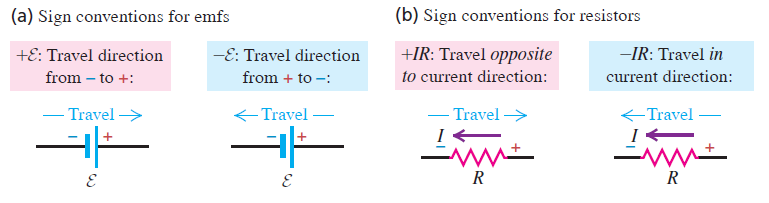
\includegraphics[scale=0.4]{images/fs_kirchoff_signs.png}

\heading{RC Circuits}

Charging: 

\[q=C\EP(1-e^{-t/RC}) \qquad i=\frac{dq}{dt}=\frac{\EP}{R}e^{-t/RC}\]

Time constant: $\tau=RC$

Discharging:

\[q=Q_0 e^{-t/RC} \qquad i=\frac{dq}{dt}=-\frac{Q_0}{RC}e^{-t/RC}\]

\sectionheading{Inductance}

\[\EP=-L\frac{di}{dt}\qquad\text{(Opposes change in current)}\]

\[V_{ab}=L\frac{di}{dt}\]

Kirchoff's law: same convention as resistor (if same direction as current, then $-L\frac{di}{dt}$)

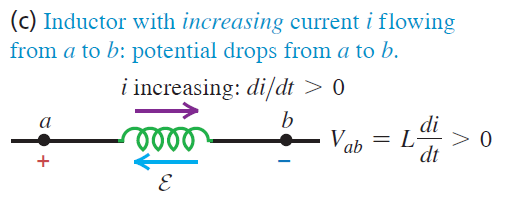
\includegraphics[scale=0.3]{images/fs_inductor_1.png}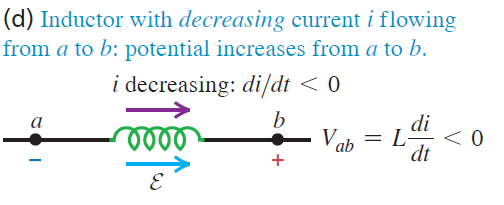
\includegraphics[scale=0.3]{images/fs_inductor_2.png}

Energy in inductor:

\[E=\frac{1}{2}LI^2\]

\heading{RL Circuits}

Current growth:

\[i=\frac{\EP}{R}(1-e^{-(R/L)t}) \qquad \frac{di}{dt}=\frac{\EP}{L}e^{-(R/L)t}\]

Time constant: $\tau=\frac{L}{R}$

Current decay:

\[i=I_0 e^{-(R/L)t}\]

\heading{LC Circuit}

Start with capacitor fully charged:

\[\omega=\frac{1}{\sqrt{LC}}\]

Capacitor: $V(t)=V_0 \cos(\frac{t}{\sqrt{LC}})=V_0\cos(\omega t)$

Inductor: $I(t)=-\frac{V_0}{\sqrt{L/C}}\sin(\frac{t}{\sqrt{LC}})=-\frac{V_0}{\sqrt{L/C}}\sin(\omega t)$

\sectionheading{RLC Circuits}

LC with damping.

\[\omega=\sqrt{\frac{1}{LC}-\frac{R^2}{4L^2}} \qquad \tau=\frac{2L}{R}\]

\[q=Q_0e^{-(R/2L)t}\cos\biggl(\sqrt{\frac{1}{LC}-\frac{R^2}{4L^2}}t+\phi\biggr)\]

\[q=Q_0e^{-t/\tau}\cos(\omega t+\phi)\]

\[i=-\frac{dq}{dt}=Q_0 e^{-t/\tau}(\omega \sin (\omega t+\phi)+\frac{1}{\tau}\cos(\omega t+\phi))\]

\heading{Limiting Behaviour}

$t\to 0^+$: $C\approx$ wire, $L\approx$ broken circuit (no change in $i$)

$t\to\infty$: $C\approx$ broken circuit, $L\approx$ wire

\sectionheading{AC Circuits}

Sinusoid voltage/current:

\[v=V\cos\omega t \qquad i=I\cos\omega t\]

RMS values 
\[I_{\text{rms}}=\frac{I}{\sqrt{2}} \qquad V_{\text{rms}}=\frac{V}{\sqrt{2}}\]

\heading{Resistors}

\[V_R=IR \qquad v_R=V_R\cos\omega t\]

$v_r$ is in phase with $i$.

\heading{Inductors}

\[V_L = IX_L \qquad X_L = \omega L \qquad v_L=V_L\cos(\omega t+90^\circ)\]

$v_L$ leads $i$ by $90^\circ$.

Inductors block high frequencies and permit low frequencies + DC to pass through (low-pass filter)

\heading{Capacitors}

\[V_C=IX_C \qquad X_C=\frac{1}{\omega C} \qquad v_C=V_C\cos(\omega t-90^\circ)\]

$v_C$ lags $i$ by $90^\circ$.

Capacitors block low frequencies + DC and permit high frequencies to pass through (high-pass filter)

\sectionheading{LRC AC Circuit}

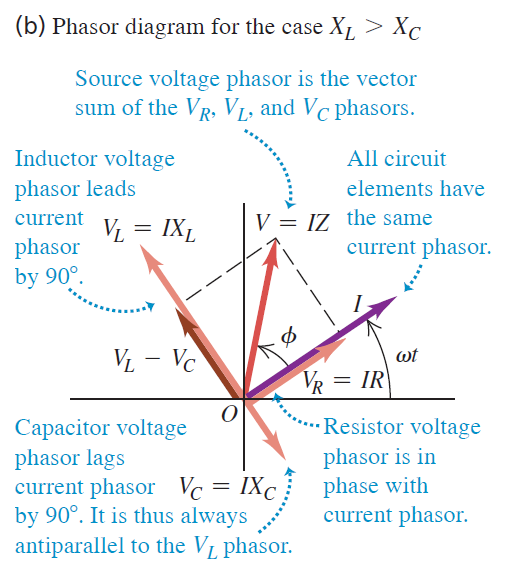
\includegraphics[scale=0.3]{images/fs_rlc_phasor_1.png}
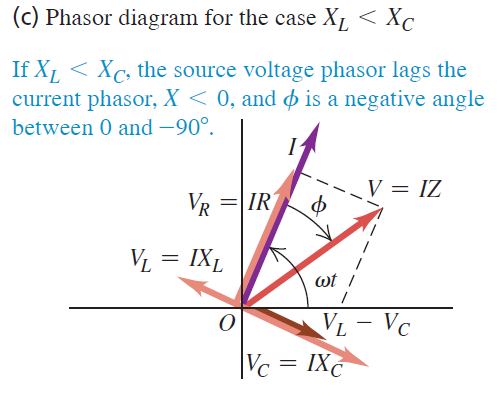
\includegraphics[scale=0.35]{images/fs_rlc_phasor_2.png}

\heading{Impedance}

\[Z=\sqrt{R^2+(X_L-X_C)^2}\]

\[V=IZ \qquad \text{(amplitudes)}\]

\[\tan\phi=\frac{X_L-X_C}{R}=\frac{\omega L-1/\omega C}{R}\]

If $i=I\cos\omega t$, then source voltage $v=V\cos(\omega t+\phi)$

\heading{Power}

Instantaneous: $p=vi$

Resistor: $P_{\text{av}}=\frac12 VI=V_{\text{rms}}I_{\text{rms}}$

Capacitor and inductor: $P_{\text{av}}=0$

General AC circuit:

\[P_{av}=\frac12 VI\cos\phi=V_{\text{rms}}I_{\text{rms}}\cos\phi\]

Power factor: $\cos\phi$

\end{multicols*}

\end{document}

